\documentclass[8pt]{beamer}
\usepackage[authoryear,round]{natbib}
\usepackage{graphicx}
\usetheme[width=2cm]{Goettingen}
\usepackage[utf8x]{inputenc}
\usepackage[T1]{fontenc}
\usepackage[french]{babel}
\usepackage[small]{caption}
%%%Présentation faite pour le seminaire du Lophiss en Octobre 2012

\author{Simon}
\title{Robotique Évolutionnaire \& Biologie }
\begin{document}

\begin{frame}
	\titlepage
\end{frame}
\section{Préambule}
\begin{frame}{Préambule}

	\vfill
	\begin{columns}
		\column{.5\textwidth}
		\begin{figure}[h]
			\begin{center}
				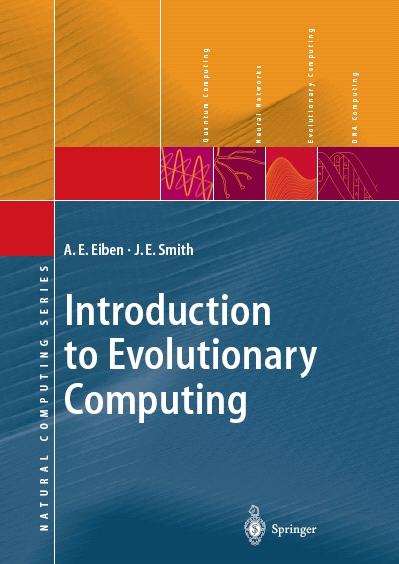
\includegraphics[height=4cm]{images/ec}
			\end{center}
			\caption{\cite{eiben03introductiontoevolutionarycomputing}}
			\label{fig:ec}
		\end{figure} 

		\vfill
		Algoritmique Évolutionaire 1970 : \cite{holland75adaptationnaturalartificialsystem}



		\column{.5\textwidth}

		\begin{figure}[h]
			\begin{center}
				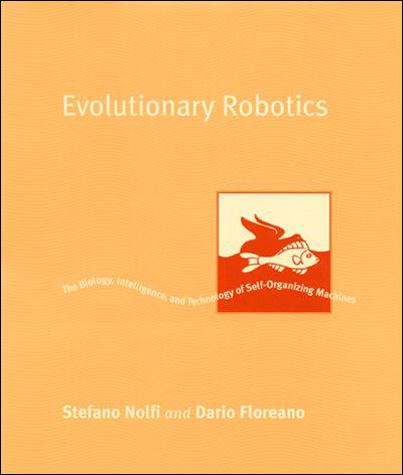
\includegraphics[height=4cm]{images/er}
			\end{center}
			\caption{\cite{nolfi00evolrobobiolintetechselfmach}}
			\label{fig:er}
		\end{figure}

		\vfill
		Robotique Évolutionnaire 1990 : \cite{nolfi00evolrobobiolintetechselfmach}
	\end{columns}
	\vfill

	$\rightarrow$ utiliser Darwin pour concevoir des systèmes artificiel
\end{frame}

\begin{frame}
	Algorithme génétique :
	\begin{figure}
		\centering
		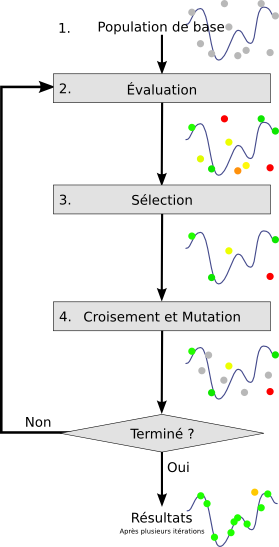
\includegraphics[width=.3\textwidth]{images/AG.png}
		\caption{Exemple d'algorithme génétique (source : wikipedia)}\label{fig:AG}
	\end{figure}
\end{frame}

\section{Évolution ``Embarquée''} 
\begin{frame}{Approche ER ``Classique''}

	\begin{columns}
		\column{.3\textwidth}
		\begin{figure}
			\centering
			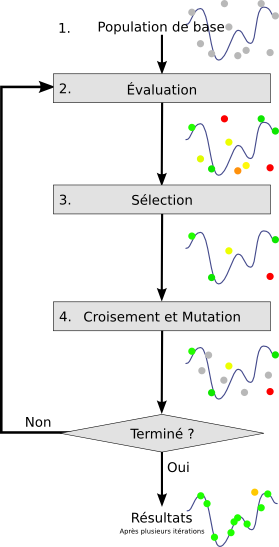
\includegraphics[width=\textwidth]{images/AG}
		\end{figure}
		\column{.65\textwidth}
		\begin{figure}
			\centering
			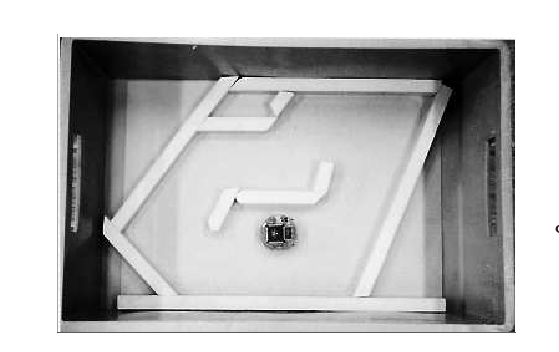
\includegraphics[width=.9\textwidth]{images/oldERfloreano}
			\caption{extrait de \cite{floreano94automaticcreationofanautonomousagen}}\label{fig:oldEr}
		\end{figure}
	\end{columns}

\end{frame}

\begin{frame}{EE}
	\begin{columns}
		\column{.5\textwidth}
		\begin{quote}
			In natural evolution the adaptative mechanism is completely decentralized and distributed: evaluation is implicit and reproduction is carried out autonomously by the agents in the population\\
			\cite[p. 2]{watson02embodiedevolutiondistributingevolutionaryalgorithmpopulationrobots}
		\end{quote}
		\column{.6\textwidth}

		\begin{figure}
			\centering
			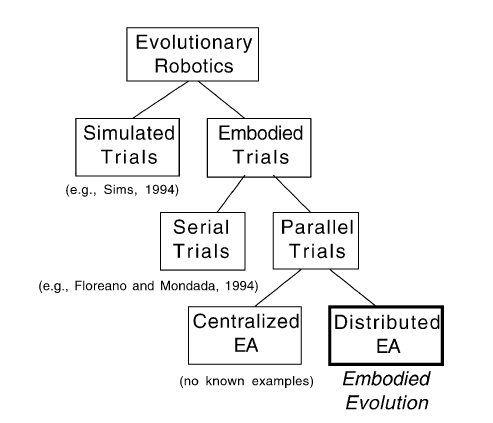
\includegraphics[width=.9\textwidth]{images/erTree.png}
			\caption{Différentes approches d'ER. Image reprise de \cite{watson02embodiedevolutiondistributingevolutionaryalgorithmpopulationrobots}}\label{fig:erTree}
		\end{figure}
	\end{columns}

	\begin{block}{Solution}
		\cite{watson02embodiedevolutiondistributingevolutionaryalgorithmpopulationrobots}: pour surpasser les pbs $\rightarrow$ Algorithme distribué sur un ensemble de robots (Alife-like cf. \cite{ray91anapproachtothesynthesisoflife}, open-ended evolution). 
	\end{block}

\end{frame}


\section{Modèles des processus évolutifs naturels?}

\begin{frame}
	De nombreuses études et exemples, notamment : \cite{bredeche11mcmds}

	Évolution ``Environment Driven''.
	
\end{frame}

	%%%----------------------------------------------------------------------
	%%%----------------------------------------------------------------------
%%%%%%%%%%%%%%%%%%%%%%%%%%%%%%%%%%%%%%%%%%%%%%%%%%%555
%From jm and nicolas frame 

  \newcommand{\mEDEA}{

	\begin{itemize}
		\item Chaque agent contient:
		\begin{itemize}
			\item un génome actif, utilisé pour contrôler l'agent,
			\item Une \emph{liste des génomes re\c cus}, utilisée pour stocker les génomes re\c cus pendant une génération,  
		\end{itemize}
		
		\item \`{A} chaque pas de temps, chaque agent :
		\begin{itemize}
			\item émet des copies dont son génome actif,
			\item stocke les génomes re\c cus des agents voisins.
		\end{itemize}
		
		\item \`{A} la fin d'une génération, chaque agent:
		\begin{itemize}
			\item "oublie" son génome actif, 
			\item choisit au hasard un génome parmis les génomes de sa \emph{liste de génomes re\c cus} comme nouveau génome actif et le mute légèrement,
			\item vide sa liste des génomes re\c cus.
		\end{itemize}
	\end{itemize}

}


%------------------------------------------------------------
\begin{frame}{L'algorithme <<mEDEA>>}
\begin{figure}
 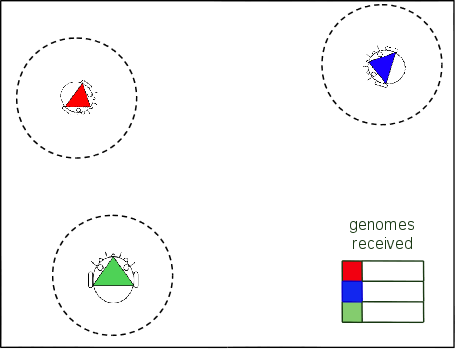
\includegraphics[height=3cm]{images/medea0}
\end{figure}

  \mEDEA

\end{frame}

%------------------------------------------------------------
\begin{frame}{L'algorithme <<mEDEA>>}\addtocounter{framenumber}{-1}
\begin{figure}
 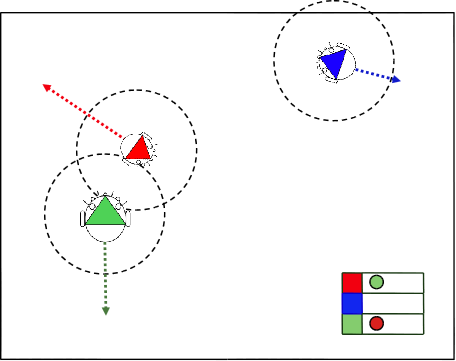
\includegraphics[height=3cm]{images/medea1}
\end{figure}
   \mEDEA
\end{frame}
%------------------------------------------------------------
\begin{frame}{L'algorithme <<mEDEA>>}\addtocounter{framenumber}{-1}
\begin{figure}
 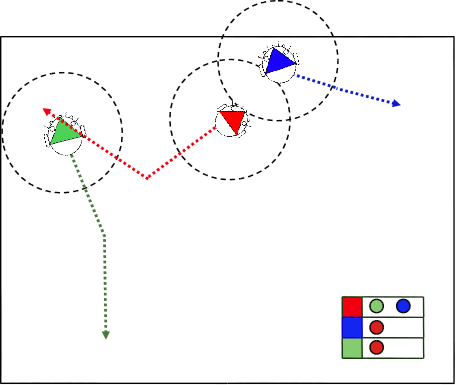
\includegraphics[height=3cm]{images/medea2}
\end{figure}
   \mEDEA
\end{frame}

%------------------------------------------------------------

\begin{frame}{L'algorithme <<mEDEA>>}\addtocounter{framenumber}{-1}
\begin{figure}
 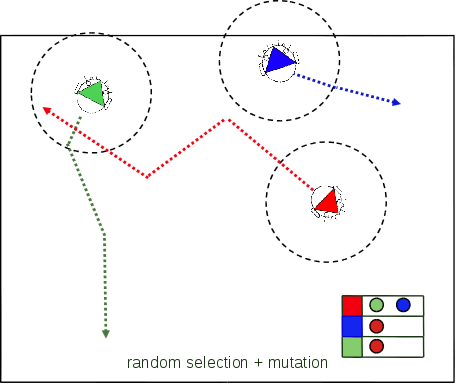
\includegraphics[height=3cm]{images/medea3}
\end{figure}
   \mEDEA
\end{frame}


%%%%%%%%%%%%%%%%%%%%%%%%%%%%%%%%%%




	%%%----------------------------------------------------------------------
	%%%----------------------------------------------------------------------
\begin{frame}{Travaux précédents}
	\begin{columns}
		\column{0.5\textwidth} 
		\begin{figure}%[h]
			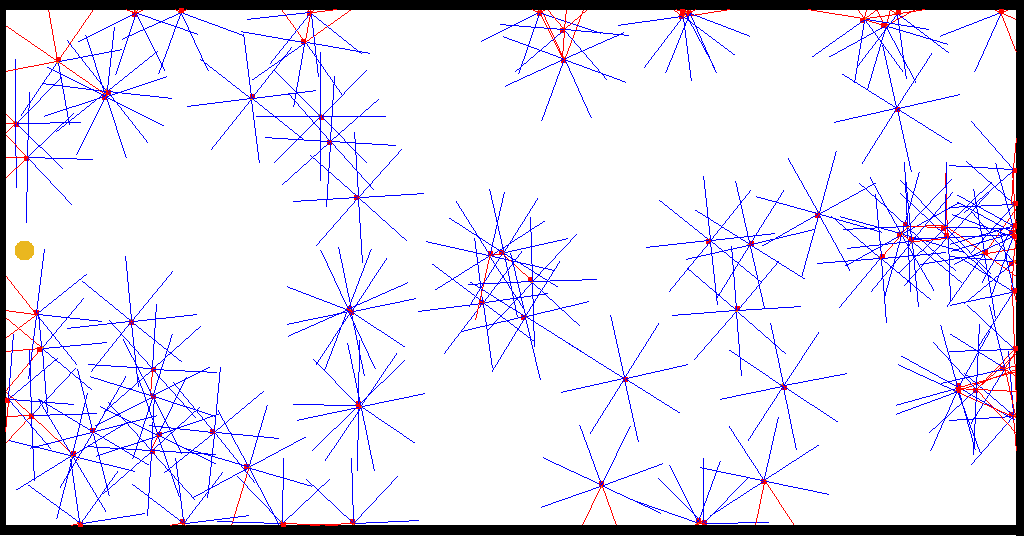
\includegraphics[width=\textwidth,height=3cm]{images/roborobo-setup-twosuns}
		\end{figure}
		\column{0.5\textwidth} 
		\begin{figure}%[h]
			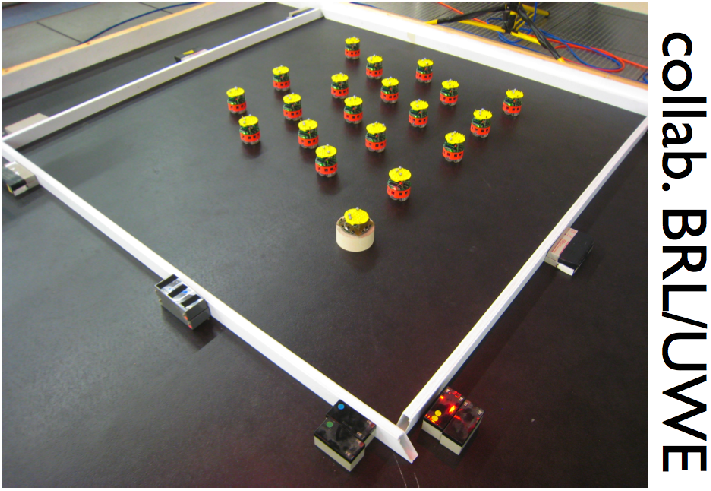
\includegraphics[width=\textwidth,height=3cm]{images/medea-RealRobots}
		\end{figure}
	\end{columns}

	\vfill

% 	Travaux précédents
	\begin{itemize}
		\item Robuste aux changements environnementaux {\small[PPSN2010]}, \nocite{bredeche11mcmds} 
			\vfil
		\item Fonctionne sur robots réels {\small[MCMDS2011]}, %\nocitep{montanier}
			\vfil
		\item \'{E}mergence de l'altruisme {\small[ECAL2011]},
			\vfil
		\item \'{E}mergence de concensus {\small[MCMDS2011]}.
	\end{itemize}

% 	\vfill

\end{frame}

\begin{frame}
	
	\begin{alertblock}{Questions}
		\begin{itemize}
			\item Valeur épsitémique de ces études?
			\item Modèles pour comprendre les mécanismes évolutifs tels qu'ils existent en biologie?
		\end{itemize}
	\end{alertblock}

	\begin{block}{Pistes}
		\begin{itemize}
			\item Argument par analogie,
			\item Expériences de pensée,
			\item Approche sémantique des théories,
			\item Vie artificielle (alife as opaque thought experiment),
			\item \dots
		\end{itemize}
	\end{block}

	
\end{frame}

\begin{frame}
	\bibliographystyle{apalike}
	\bibliography{/home/simon/Documents/biblio/memoireLophiss}
\end{frame}

\end{document}

